\chapter{Resultados}

Este capítulo presenta los resultados obtenidos con el sistema descrito en el capítulo anterior, y los contrasta con los objetivos y la motivación planteados en la introducción. La evaluación se organiza en cuatro capas complementarias, ordenadas por coste y profundidad, seguidas de una discusión que conecta lo observado con las preguntas de investigación. Las capas 1 y 2 están implementadas de forma completa. La capa 3 está implementada de forma preliminar para un subconjunto de escenarios y modelos. La capa 4 se aplicó como revisión manual exploratoria, y su versión formal con doble anotación independiente queda como trabajo futuro.

\section{Capa 1: Aserciones estructurales}

La primera capa verifica que la salida del pipeline cumple condiciones básicas con independencia del contenido del hilo. Antes de que el resultado salga del pipeline se comprueba que la respuesta no está vacía, que la técnica pertenece al repertorio conocido, que el valor de confianza está en el rango válido y que las flags de escalado al instructor y de publicación en el hilo son coherentes entre sí; durante la generación del texto, el agente de rol detecta presencia de lenguaje evaluativo y técnica no especificada. Cuando cualquiera de estas comprobaciones falla, el sistema activa el circuito de retroalimentación y reintenta la generación con el feedback incluido en el contexto, hasta un máximo de tres intentos.

Estas comprobaciones no son suficientes para determinar si una respuesta es pedagógicamente adecuada. Una respuesta puede pasar todas las verificaciones y seguir siendo inapropiada si la técnica está mal aplicada al contexto o el texto no está fundamentado en las contribuciones del hilo. Para eso están las capas siguientes.

\section{Capa 2: Evaluación con escenarios de prueba}

La segunda capa evalúa el comportamiento del sistema contra ocho escenarios de discusión definidos en código, en \texttt{discussion\_moderation/evals/fixtures/}, y ejecuta el pipeline de forma reproducible contra cada uno.

Seis escenarios cubren uno a uno los estados de la taxonomía (nueva, activa, estancada, conflictiva, convergente y fuera de tema), diseñados para que el clasificador los asigne sin ambigüedad. De esos seis, solo dos producen intervención; dos escenarios adicionales cubren ese espacio. El primero representa un hilo con participación distribuida pero discurso formulaico, donde ningún estudiante desarrolla argumentos ni conecta ideas con las lecturas del curso, y activa el rol intelectual. El segundo representa un hilo donde un participante domina la discusión con varias contribuciones sustantivas y el resto solo asiente brevemente, y activa el rol social. Todos los escenarios comparten el mismo contexto de curso y una marca de tiempo fija para que los resultados sean comparables entre modelos y entre fechas.

La herramienta registra la clasificación obtenida, la decisión de intervención, el rol seleccionado si hubo intervención y si la respuesta superó la validación. Esta capa verifica que el modelo completa el pipeline sin errores y que sus clasificaciones son coherentes con el estado diseñado para cada escenario, pero no evalúa la calidad pedagógica de las respuestas.

Los experimentos descritos en este apartado se ejecutaron el 14 de junio de 2026 contra los ocho escenarios con dos modelos externos (\texttt{openrouter:openai/gpt-4o} y \texttt{openrouter:anthropic/claude-sonnet-4.5}) y un modelo local en Idril (\texttt{ollama:ministral-3:14b}). La tabla~\ref{tab:resultados-fixtures} recoge los resultados obtenidos para cada escenario.

\begin{table}[h]
\centering
\small
\begin{tabular}{llllllll}
\toprule
\textbf{Escenario} & \textbf{Estado esperado} & \multicolumn{2}{c}{\textbf{gpt-4o}} & \multicolumn{2}{c}{\textbf{claude-sonnet-4.5}} & \multicolumn{2}{c}{\textbf{ministral-3-14b}} \\
 & & Estado & Interviene & Estado & Interviene & Estado & Interviene \\
\midrule
new              & nueva         & nueva       & sí   & estancada   & sí & nueva      & no \\
active           & activa        & activa      & no   & estancada   & sí & activa     & no \\
stalled          & estancada     & nueva       & no   & estancada   & sí & estancada  & sí \\
conflictive      & conflictiva   & conflictiva & sí   & conflictiva & sí & conflictiva & sí \\
convergent       & convergente   & activa      & no   & estancada   & sí & convergente & no \\
off\_topic       & fuera de tema & fuera de tema & sí & fuera de tema & sí & —         & — \\
shallow\_discourse & superficial  & convergente & no   & estancada   & sí & estancada & sí \\
dominated        & dominada      & estancada   & no   & —           & — & estancada & no \\
\midrule
\textbf{Correctos} & & \textbf{4/8} & \textbf{4/8} & \textbf{3/7} & \textbf{4/7} & \textbf{5/8} & \textbf{7/8} \\
\bottomrule
\end{tabular}
\caption{Clasificación e intervención sobre los ocho escenarios de prueba. — indica ejecución incompleta. Correcto: valor obtenido coincide con el esperado.}
\label{tab:resultados-fixtures}
\end{table}

Adicionalmente se ejecutó un experimento contra seis hilos reales del curso \texttt{course-v1:openedx+PROG+2026}, recogidos directamente de la instancia de Open edX. La tabla~\ref{tab:resultados-lms} muestra la clasificación y la decisión de intervención producidas por cada modelo para cada hilo. En este caso no existe estado esperado definido, ya que los hilos provienen de actividad real de estudiantes.

\begin{table}[h]
\centering
\small
\begin{tabular}{p{4.8cm}llll}
\toprule
\textbf{Hilo} & \multicolumn{2}{c}{\textbf{gpt-4o}} & \multicolumn{2}{c}{\textbf{claude-sonnet-4.5}} \\
 & Estado & Rol & Estado & Rol \\
\midrule
Extensión de plazo (anuncio) & estancada & afectivo & fuera de tema & — \\
Peer assessment (conflicto) & conflictiva & moderador & conflictiva & moderador \\
Test demasiado difícil       & estancada & organizacional & conflictiva & organizacional \\
¿Cómo obtuvimos 59?          & convergente & — & estancada & intelectual \\
Error en el examen semana 1  & nueva & organizacional & fuera de tema & — \\
Knowing vs Doing             & conflictiva & — & estancada & intelectual \\
\bottomrule
\end{tabular}
\caption{Clasificación y rol sobre seis hilos reales del curso PROG 2026. — indica no intervención.}
\label{tab:resultados-lms}
\end{table}

\begin{figure}[!ht]
\centering
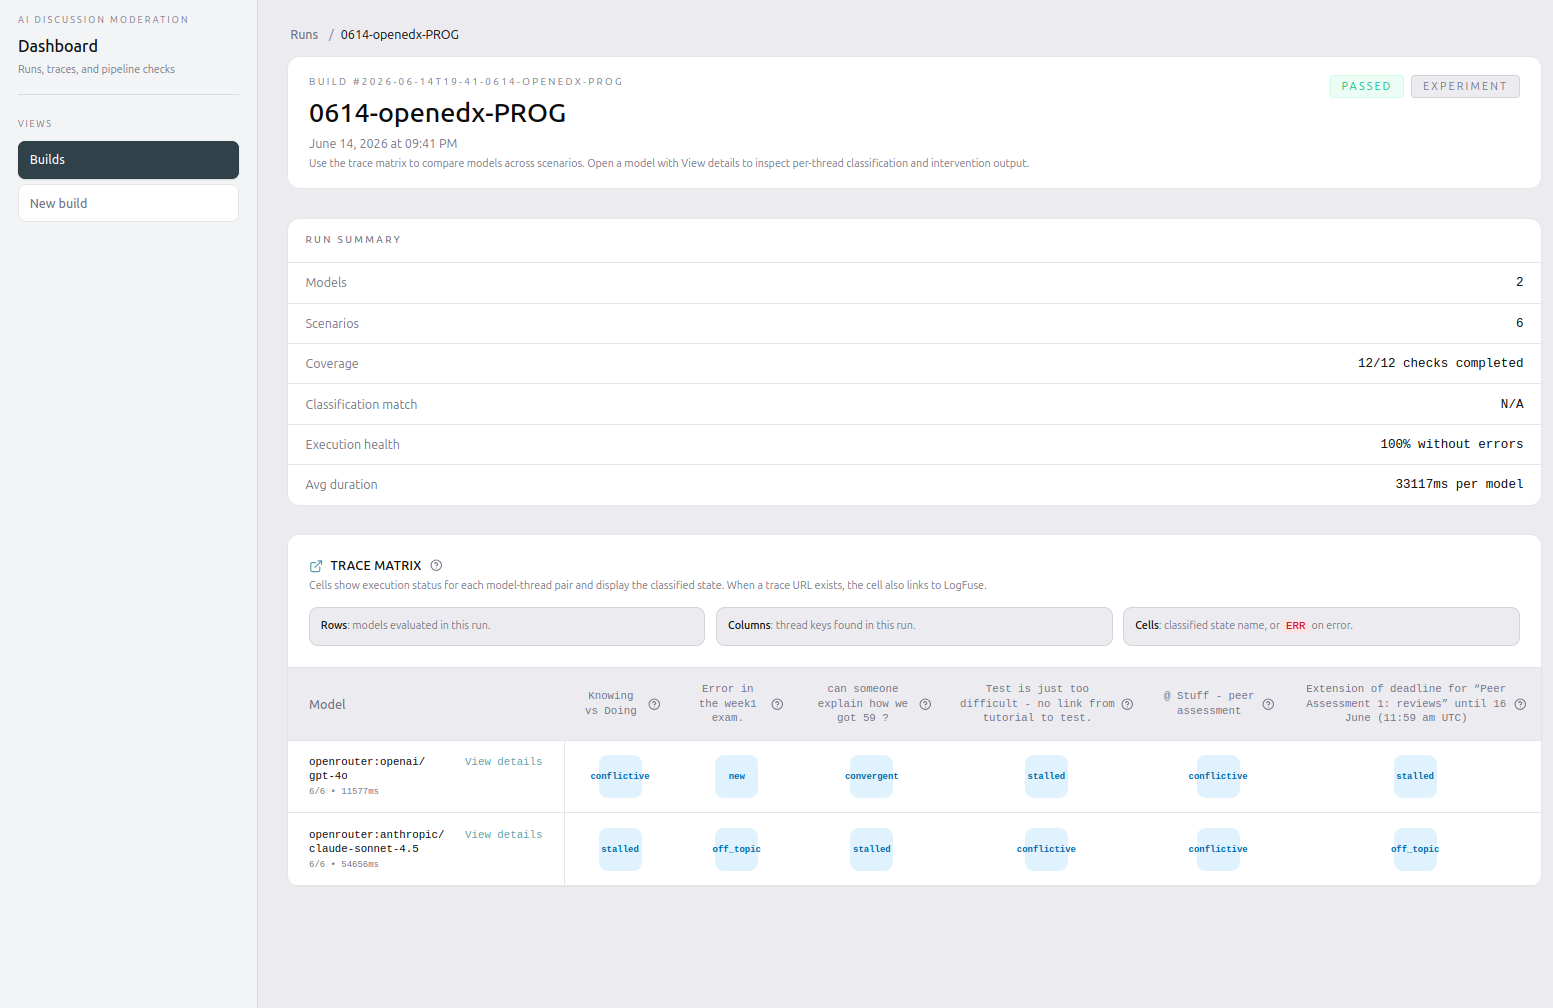
\includegraphics[width=0.9\textwidth]{figures/dashboard-trace-lms}
\caption{Matriz de trazas del run PROG: dos modelos × seis hilos reales del curso.}
\label{fig:dashboard-trace-lms}
\end{figure}

La tabla~\ref{tab:costes-experimentos} recoge el desglose de coste y uso de tokens por modelo para el conjunto de experimentos del 14 de junio.

\begin{table}[h]
\centering
\small
\begin{tabular}{lrrrrr}
\toprule
\textbf{Modelo} & \textbf{Llamadas} & \textbf{Tokens entrada} & \textbf{Tokens salida} & \textbf{Latencia media} & \textbf{Coste total} \\
\midrule
gpt-4o              & 61 & 162.229 & 8.733  & 1,7 s  & \$0,49 \\
claude-sonnet-4.5   & 60 & 237.761 & 31.349 & 12,2 s & \$1,18 \\
ministral-3-14b (Idril) & 8 & 58.012 & 11.306 & 82,8 s & N/A (local) \\
\midrule
\textbf{Total OpenRouter}      & 121 & 399.990 & 40.082 & — & \$1,68 \\
\bottomrule
\end{tabular}
\caption{Coste y uso de tokens por modelo, experimentos del 14 de junio de 2026.}
\label{tab:costes-experimentos}
\end{table}

El panel de evaluación descrito en el capítulo anterior permite lanzar experimentos, filtrar resultados por modelo o escenario e inspeccionar trazas desde el navegador sin necesitar acceso SSH a ninguno de los dos entornos.

\section{Capa 3: Clasificación automática con LLM}

La tercera capa aplica una clasificación automática con LLM sobre las salidas del pipeline para verificar coherencia entre estado del hilo, decisión de intervención y rol seleccionado. En esta capa se registra si la salida es consistente con la taxonomía de estados definida y si la decisión tomada corresponde al patrón de participación observado en el hilo. En este trabajo, esta capa se aplicó de forma preliminar sobre un subconjunto de pares modelo-hilo para detectar fallos sistemáticos de clasificación y de selección de rol.

\section{Capa 4: Revisión manual y anotación por expertos}

En la ejecución actual se realizó una revisión manual exploratoria de salidas para contrastar la clasificación automática y verificar coherencia entre estado clasificado, técnica seleccionada y tono de la intervención. Para eso se usaron dos herramientas. El panel de evaluación permite inspeccionar el contenido del hilo y la intervención generada en una sola vista. Logfire expone la traza completa de cada ejecución, incluyendo los mensajes enviados a cada agente y sus respuestas. Esta revisión permitió identificar errores de aplicación de técnica y casos límite no detectados por aserciones estructurales.

\begin{figure}[!ht]
\centering
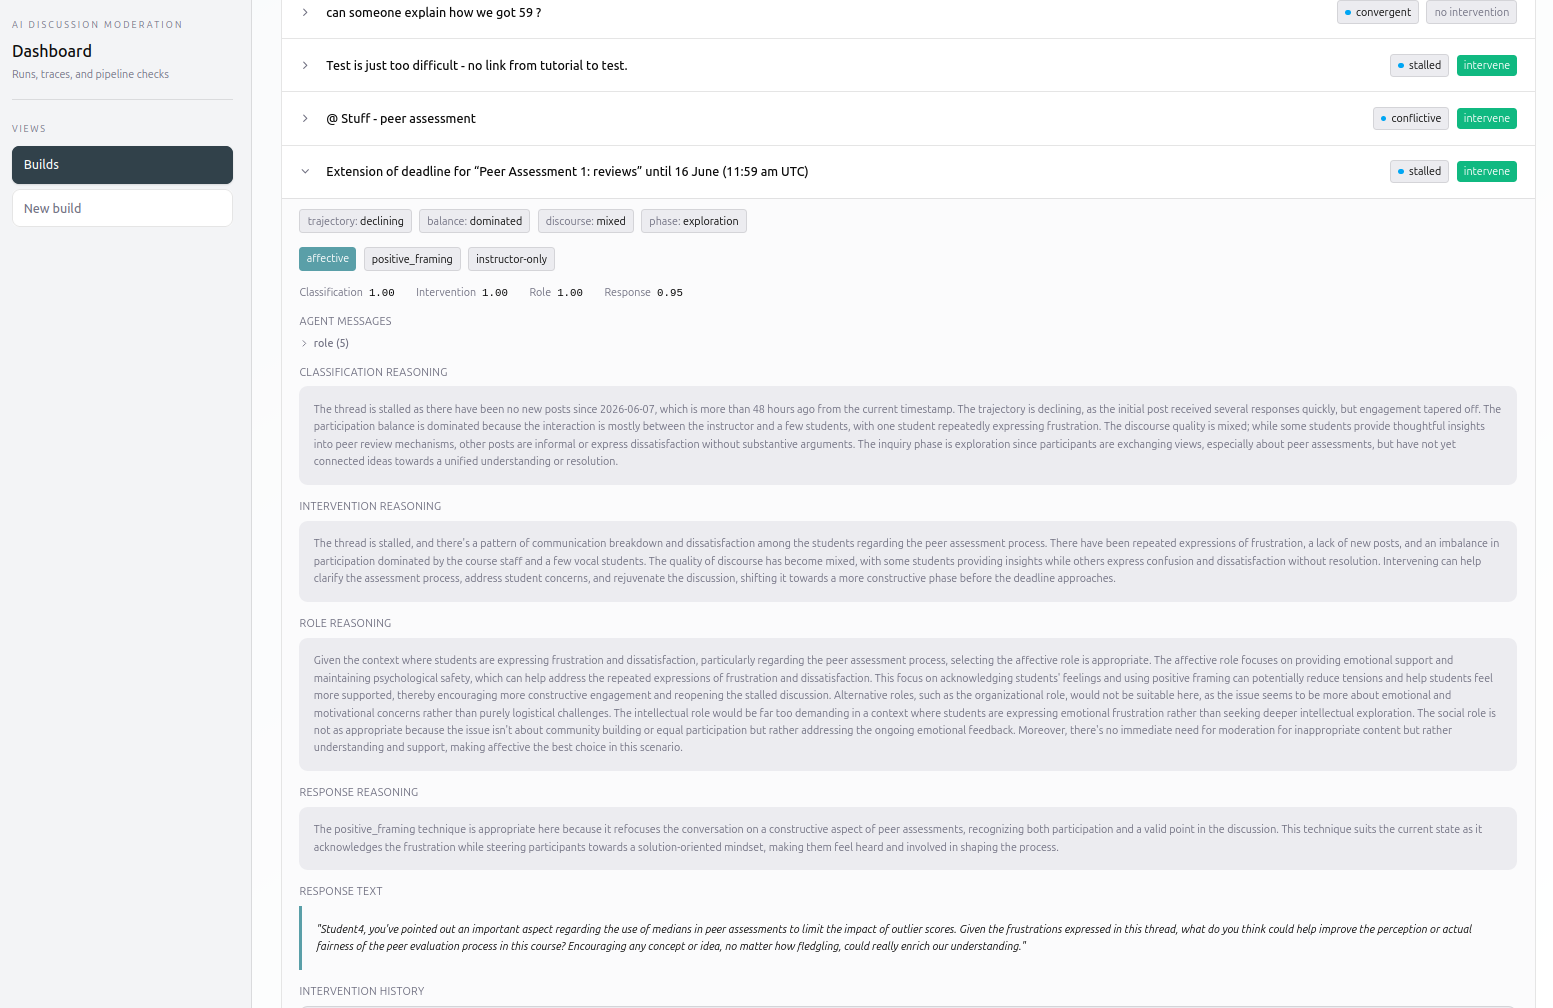
\includegraphics[width=0.85\textwidth]{figures/dashboard-thread-detail}
\caption{Detalle de un hilo en el panel: contenido, clasificación e intervención generada.}
\label{fig:dashboard-thread-detail}
\end{figure}

\begin{figure}[!ht]
\centering
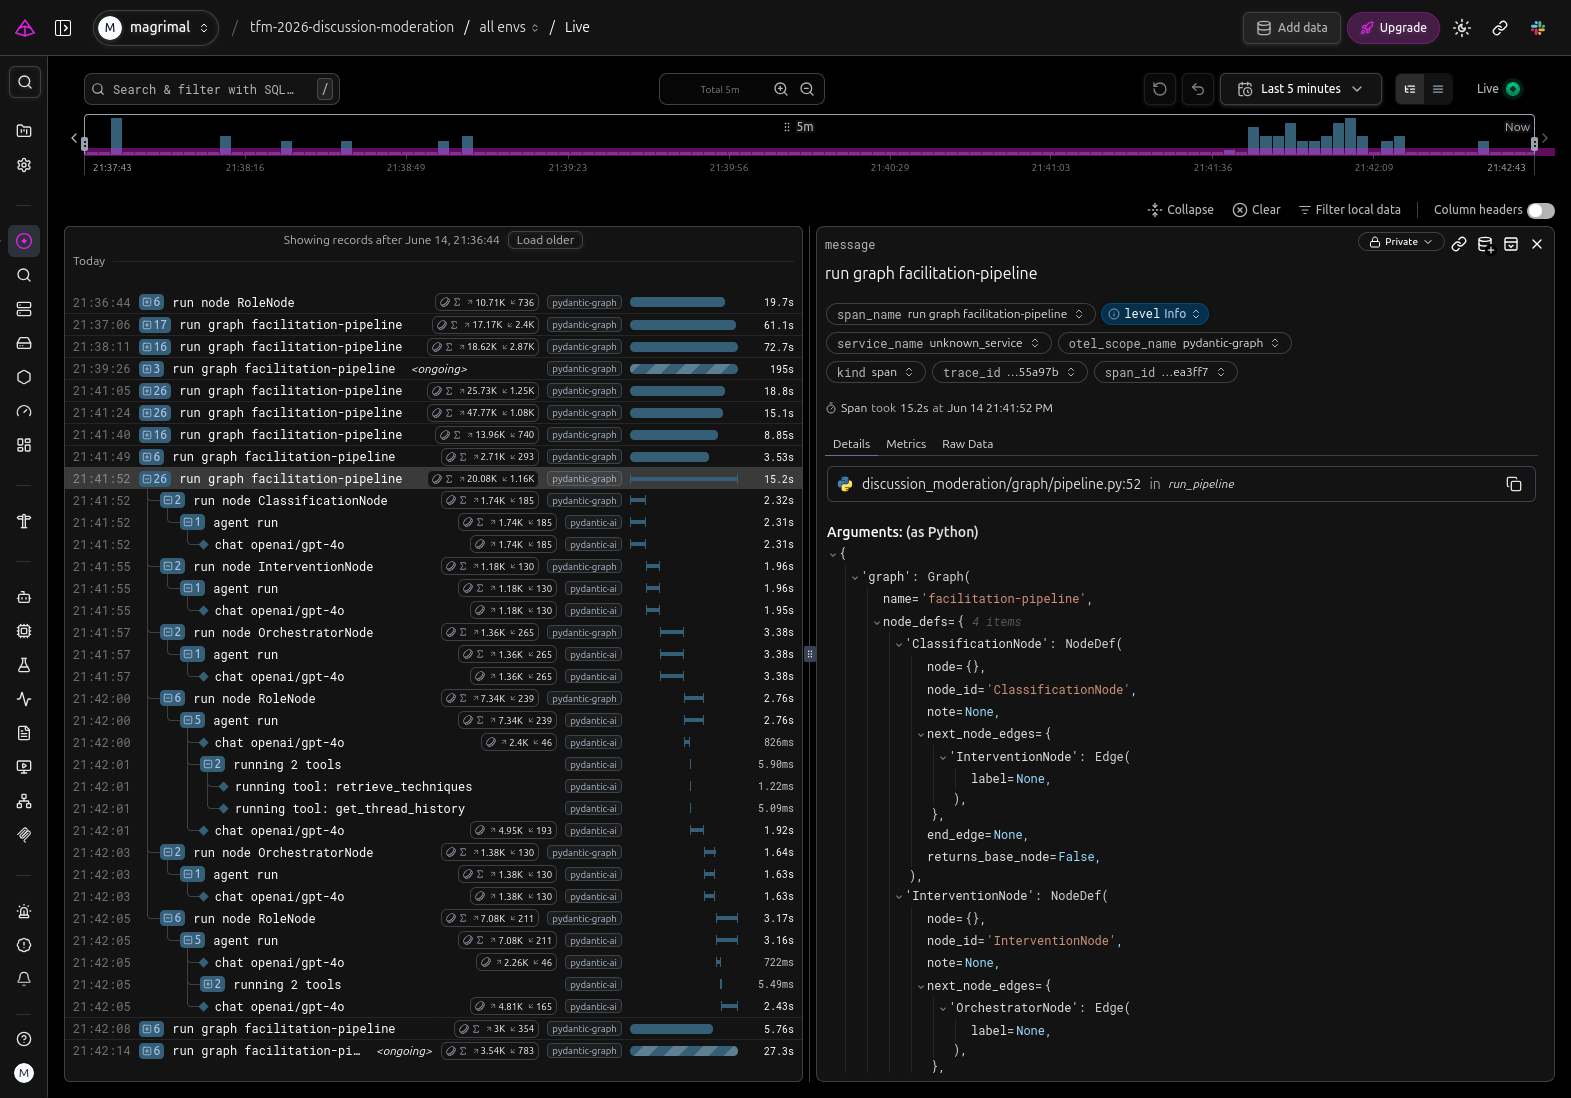
\includegraphics[width=0.85\textwidth]{figures/logfire-trace}
\caption{Trazas del pipeline de facilitación en Logfire.}
\label{fig:logfire-trace}
\end{figure}

La versión formal de esta capa, con anotación de veinte a treinta pares (hilo, respuesta) por dos anotadores independientes, cálculo de acuerdo inter-anotador mediante kappa de Cohen y resolución por consenso de desacuerdos, se define como trabajo futuro.

\section{Ejemplos de intervención}

\textit{Pendiente: esta sección debe incluir dos o tres ejemplos completos de intervención (hilo de entrada, clasificación producida y texto generado) que ilustren cada rol de facilitación, extraídos de una ejecución real del panel de evaluación. Queda pendiente de la ejecución de nuevos experimentos.}

\section{Discusión}

Los resultados de las capas 1 y 2 muestran que el pipeline completa su ciclo de clasificación, decisión e intervención de forma consistente, pero también que la precisión de clasificación varía sustancialmente entre modelos, de 3/7 a 7/8 escenarios correctos según el modelo evaluado. Esta variación responde directamente al primer objetivo específico del trabajo, producir intervenciones coherentes con el tema y la continuidad de la discusión dentro de tiempos y consumo de recursos razonables, y muestra que ese objetivo depende tanto del diseño del pipeline como de la elección de modelo, no solo del primero.

La tabla de hilos reales del curso PROG 2026 confirma que el sistema opera sobre discusiones no controladas, aunque sin estado esperado no es posible calcular una tasa de acierto sobre esos casos; la discrepancia entre modelos en la misma tabla (por ejemplo, \textit{Test demasiado difícil} clasificado como estancada por un modelo y como conflictiva por otro) es evidencia de que la clasificación de estado sigue siendo la etapa más sensible del pipeline, consistente con lo observado en los escenarios de prueba.

La tabla de costes muestra que la latencia del modelo local en Idril (82,8 s de media) es incompatible con un ciclo de facilitación interactivo, mientras que los modelos externos completan el ciclo en segundos a un coste bajo por intervención (entre \$0,008 y \$0,02 por llamada). Esta diferencia justifica la separación de entornos descrita en el capítulo anterior, experimentación con modelos locales en un entorno, facilitación en producción con modelos externos en otro.

En conjunto, la evidencia reunida en este capítulo respalda una afirmación acotada, el artefacto produce clasificaciones e intervenciones coherentes y auditables en escenarios controlados y sobre hilos reales, con una fiabilidad de clasificación que depende del modelo. No respalda una afirmación de efectividad pedagógica ni de impacto en aprendizaje, que exige la validación con estudiantes reales descrita como trabajo futuro en las conclusiones.
